\documentclass{beamer}
\usetheme{Dresden}
\setbeamercovered{transparent}
%Use this to create handouts without gradual uncovering of text on each slide:
%\documentclass[handout]{beamer}

%Bibtex
\usepackage[authoryear]{natbib}
\usepackage{natbib}
\bibliographystyle{econometrica}

\usepackage{lipsum}
\newcommand\Fontvi{\fontsize{4}{7.2}\selectfont}

%Dansk opsaetning
\usepackage[utf8]{inputenc} 
\usepackage[danish]{babel} 
\renewcommand{\danishhyphenmins}{22} 
\usepackage[T1]{fontenc}
\usepackage{amsmath, mathtools, natbib, graphicx, placeins, tabularx,booktabs}

%
\newtheorem{thm}{Sætning}
\usepackage[danish=quotes]{csquotes}

\title[DONG]{En Ex Ante Evaluering af DONG Aftalen}
\author{Niels-Jakob Harbo Hansen og Guan Yang}

%\date{\timestamp}

\begin{document}

\begin{frame}
\maketitle
\end{frame}

\section{Introduction}
\subsection{}

\begin{frame}{Introduktion}

\begin{itemize}

\item Spørgsmål: Var 2014 aftalen økonomisk set fornuftig for staten?
\pause
\item Svar: Nej 
\pause
\begin{itemize}
\item I et offentligt alternativ, have opnået et forventet afkast på 2 mia.\ udover hvad man opnåede med den indgåede aftale.
\pause
\item  Sandsynligheden for at den indgåede aftale giver et bedre afkast end det offentlige alternativ er cirka 60 \%, men  afkaststruktur stærkt asymmetrisk.
\pause
\item Aktieprisen de private investorer betalte for DONG's egenkapital var reelt ikke var 107 DKK men derimod cirka 86 DKK. \end{itemize} 

\end{itemize}

\end{frame}

\begin{frame}{Papiret i en figur}

\begin{figure}
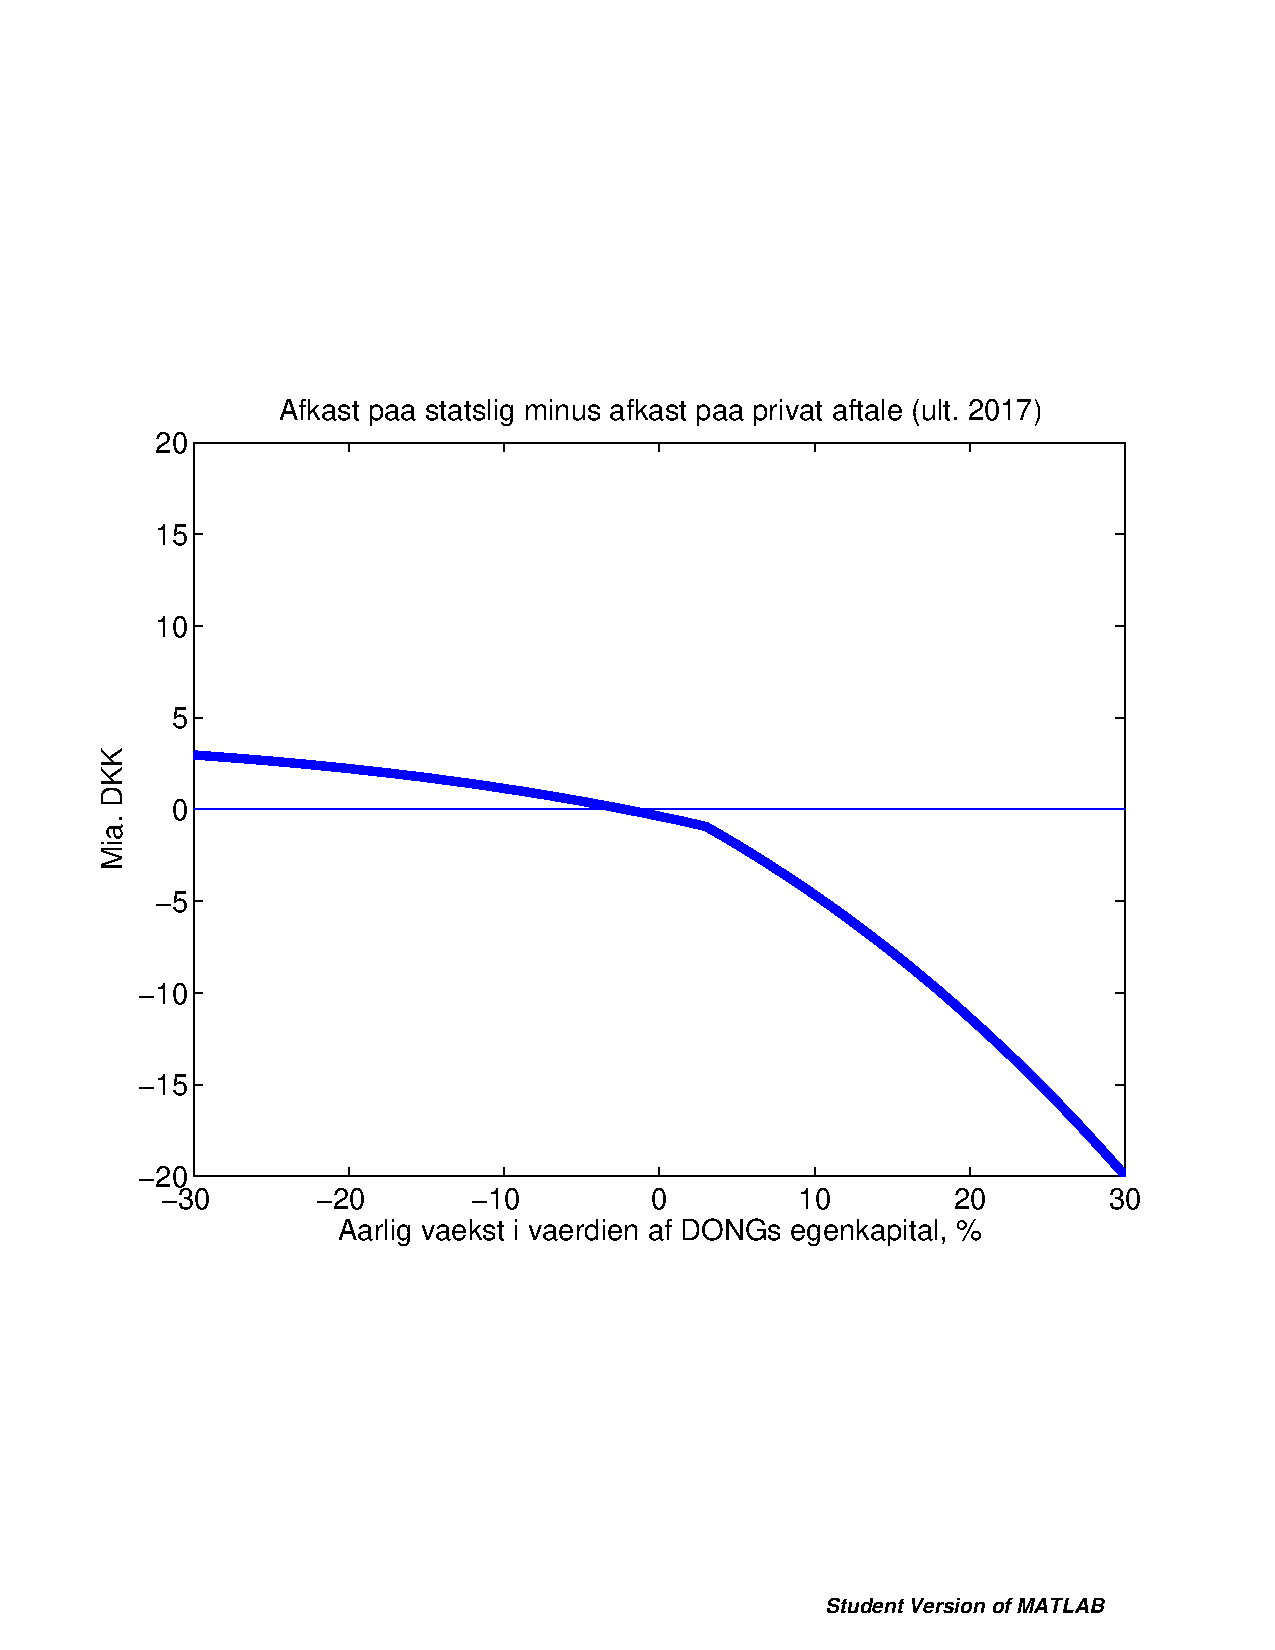
\includegraphics[scale=0.35]{../../matlab/Samfundsokonom/figs/private_less_public_deal}
\caption{\footnotesize Illustration af forskellen mellem statens absolutte afkast på den indgåede private aftale og den alternative offentlig aftale som funktion af den årlige vækst i DONGs egenkapital. }
\label{fig:comp}
\end{figure}

\end{frame}


\section{Aftalen}
\subsection{}

\begin{frame}{2014 aftalen, I}

\begin{itemize}

\item En kapitaludvidelse i DONG på 11 mia. 
\pause
\item Nye aktionærer fik put-option, som under visse omstændigheder giver investorerne ret til at sælge deres aktier til staten til
\pause
\begin{enumerate}
\item markedsprisen  eller
\pause
\item markedsprisen for 40\% af aktierne og 60\% af aktierne forrentet med den årlige CITA rente, baseret på rentekurven ultimo 2013, tillagt 2.25\%.
\end{enumerate}
\end{itemize}

\end{frame}

\begin{frame}{2014 aftalen, I}

\begin{figure}
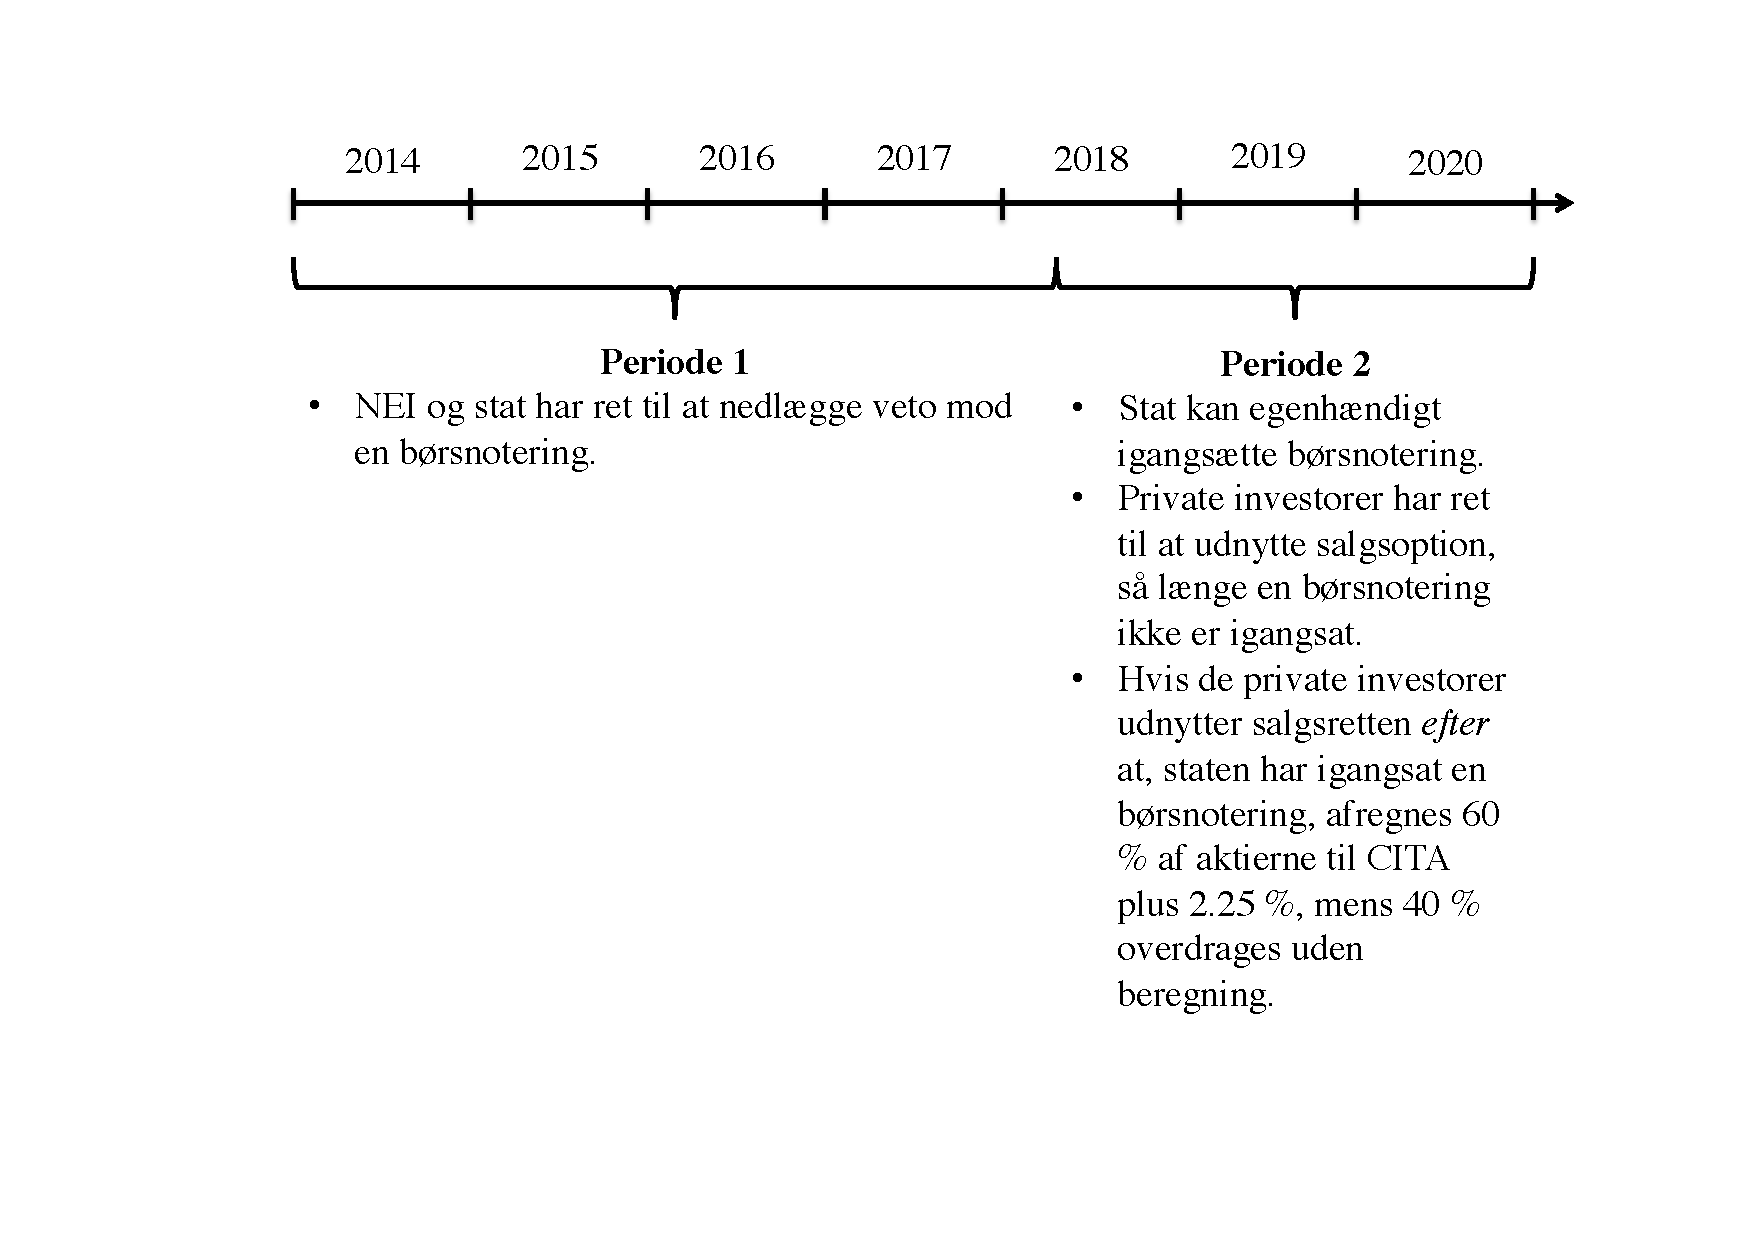
\includegraphics[scale=0.35]{../../figs/perioder}
\caption{Illustration af perioder i statens aftale med de private investorer. Kilde: \citet{FM2013a}}
\label{fig:comp}
\end{figure}
\end{frame}





\begin{frame}{Hvornår udnyttes salgsretten?}

\begin{itemize}
	
	\item \textbf{Salgsretten udnyttes primo 2018, hvis markedsværdi $<$ pris i salgsret.}

\item Indse igennem \emph{backwards induktion}. 

\begin{itemize}

\item Markedspris < pris i salgsret. Stat igangsætter børsnotering. Private investorer udnytter salgsret før stat igangsætter børsnotering.

\item Markedspris > pris i salgsret. Børsnotering eller stat overtager investorernes aktier til markedspris.

\end{itemize}

\end{itemize}

\end{frame}

\begin{frame}{Statens afkast på aftalen}

\begin{itemize}

\item Investorerne udnytter salgsretten hvis
\begin{align}
0.6K\prod_{i=2014}^{2017}(1+g_i)+0.4K(1+r)^n>K(1+r)^n 
\end{align}
\pause
\item Statens afkast på aftalen bliver dermed

\begin{align}
\footnotesize
P= 
\begin{dcases} 
-0.6K \prod_{i=2014}^{2017} (1+g_i)+0.6K(1+r)^n &\text{     hvis    (1) er sand} \\ %0.6\prod_{i=2014}^{2017}(1+g_k) \\&+0.4(1+r)^n>(1+r)^n \\ 
0  &\text{   ellers }
\end {dcases}
\label{eq:Goldman_deal}
\end{align}

\end{itemize}
\end{frame}

\begin{frame}{Statens afkast på aftalen}

\begin{figure}
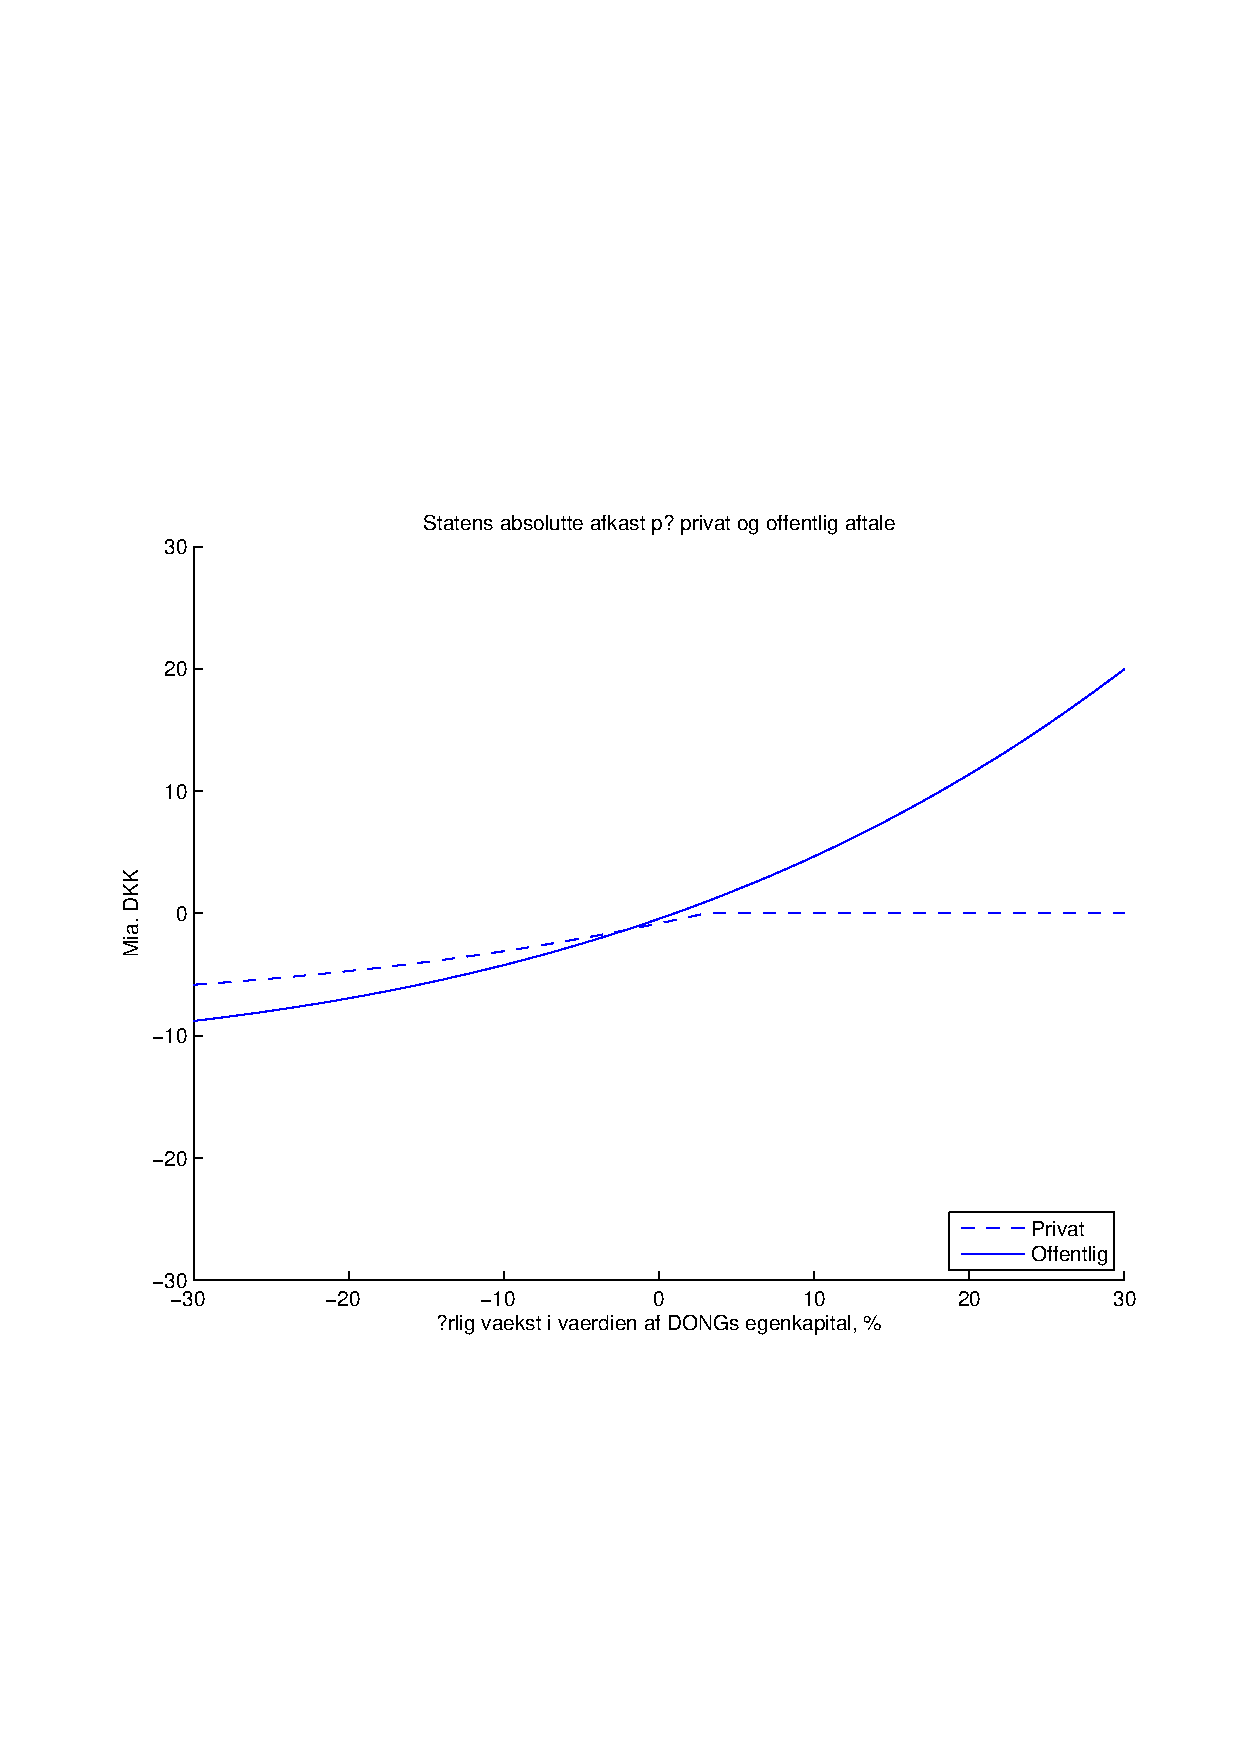
\includegraphics[scale=0.35]{../../matlab/Samfundsokonom/figs/private_public_deal}
\caption{Illustration af statens absolutte afkast henholdsvis  den indgåede private aftale og en alternativ offentlig aftale som funktion af den årlige vækst i DONGs egenkapital. }
\label{fig:privat_off}
\end{figure}


\end{frame}

\section{Evaluering}
\subsection{}

\begin{frame}{Var et en fornuftigt aftale for staten?}
	\begin{enumerate}
		\item Blev DONG handlet til en fair pris?
		\pause
		\item Dominerer aftalen i forventet afkast alle statens \emph{outside options}? 
	\end{enumerate}
\end{frame}

\begin{frame}{Hvad pris blev DONG handlet til?}

\begin{itemize}
	\item Ifølge både DONG og Finansministeriet blev DONG's eksisterende aktiekapital handlet til 107.25 DKK per aktie 
	\item $\Rightarrow$ 31.5 mia. 
	\pause
	\item Reel handelspris?
\begin{align}
\text{107.25 DKK} &= \text{aktie + option på 60\% af aktien} \nonumber \\
\Rightarrow \text{Aktie} &= \text{107.25 DKK - option på 60\% af aktien  }
\end{align}
\end{itemize}

\end{frame}

\begin{frame}{Hvad var optionens pris?}
	
	\begin{align}
C(s,t)&=N(d_1)S-N(d_2)K \exp^{-r(T-t)} \\
d_1&= \frac{1}{\sigma\sqrt{T-t}}\left( \ln\left( \frac{S}{K} \right)+\left(r+\frac{\sigma^2}{2} \right)(T-t) \right) \nonumber \\
d_2&=d_1-\sigma \sqrt{T-t} \nonumber
\end{align}
	\begin{itemize}
		\item $T-t=4$
		\item $S=$ 107.25 DKK - optionsværdien af de 60\% af aktien
	\item $K=$ er $S$ forrentet med CITA renten plus 2.25\%
	\item $r=0.01$
\end{itemize}

\end{frame}

\begin{frame}{Hvad var optionens pris?}

\begin{itemize}
	\item Optionspris = 21 DKK per aktie
	\item Aktiepris = 107,25
	\item \textbf{DONG  prissat til 24.1 mia. $\neq$ 31 mia.}
\end{itemize}
	
\end{frame}

\begin{frame}{Blev DONG solgt billigt?}
\begin{table}[h]
	\caption{Markedspris som pct. af bogført værdi.}
	\label{tab:bookval}
	\begin{tabularx}{\linewidth}{lXlrcccr}
	\toprule[1pt]
	Selskab && Land & Price/book \\
	\hline 
	%\emph{Ekslusiv 2014 data} \\
	%\midrule
		CEZ && Tjekkiet &  120 \% \\
		DRAX && Storbritanien &  130 \% \\
		EDF && Frankrig &  90 \%  \\
		%EON &&  &  \% \\
		Fortum && Finland &  140 \% \\
		GDF && Frankrig &  80 \% \\
		Iberdrola && Spanien &  100 \% \\
		RWE &&  Tyskland &  130 \% \\
		Verbund && Østrig &  100 \% \\
		\textbf{DONG} && \textbf{Danmark} & \textbf{61/47 \%} \\
		\bottomrule[1pt]
	\end{tabularx}
	\begin{minipage}{\linewidth}
		\footnotesize{Noter: Data er fra \texttt{http://financials.morningstar.com/valuation/price-ratio.html}. Primo 2014}
	\end{minipage}
\end{table}
\end{frame}

\begin{frame}{Var den private  aftale den bedste mulighed?}
	\begin{itemize}
		\item Offentligt alternativ
		
		\begin{align}
		P=K(1+r)^n-K(1+r_{gov})^n
		\label{eq:gov_capital}
		\end{align}
		
		\item er er $r$ den gennemsnitlige reale vækst i værdien af DONG's egenkapital i perioden 2014-17, 
		\item $n=4$, 
		\item $r_{gov}$ = 1 \% fratrukket en forventet årlig inflation på 0.5 \%
		\item Stat og private køber til markedpris 
	\end{itemize}

\end{frame}

\begin{frame}{Var den private  aftale den bedste mulighed?}
\begin{figure}
\centering
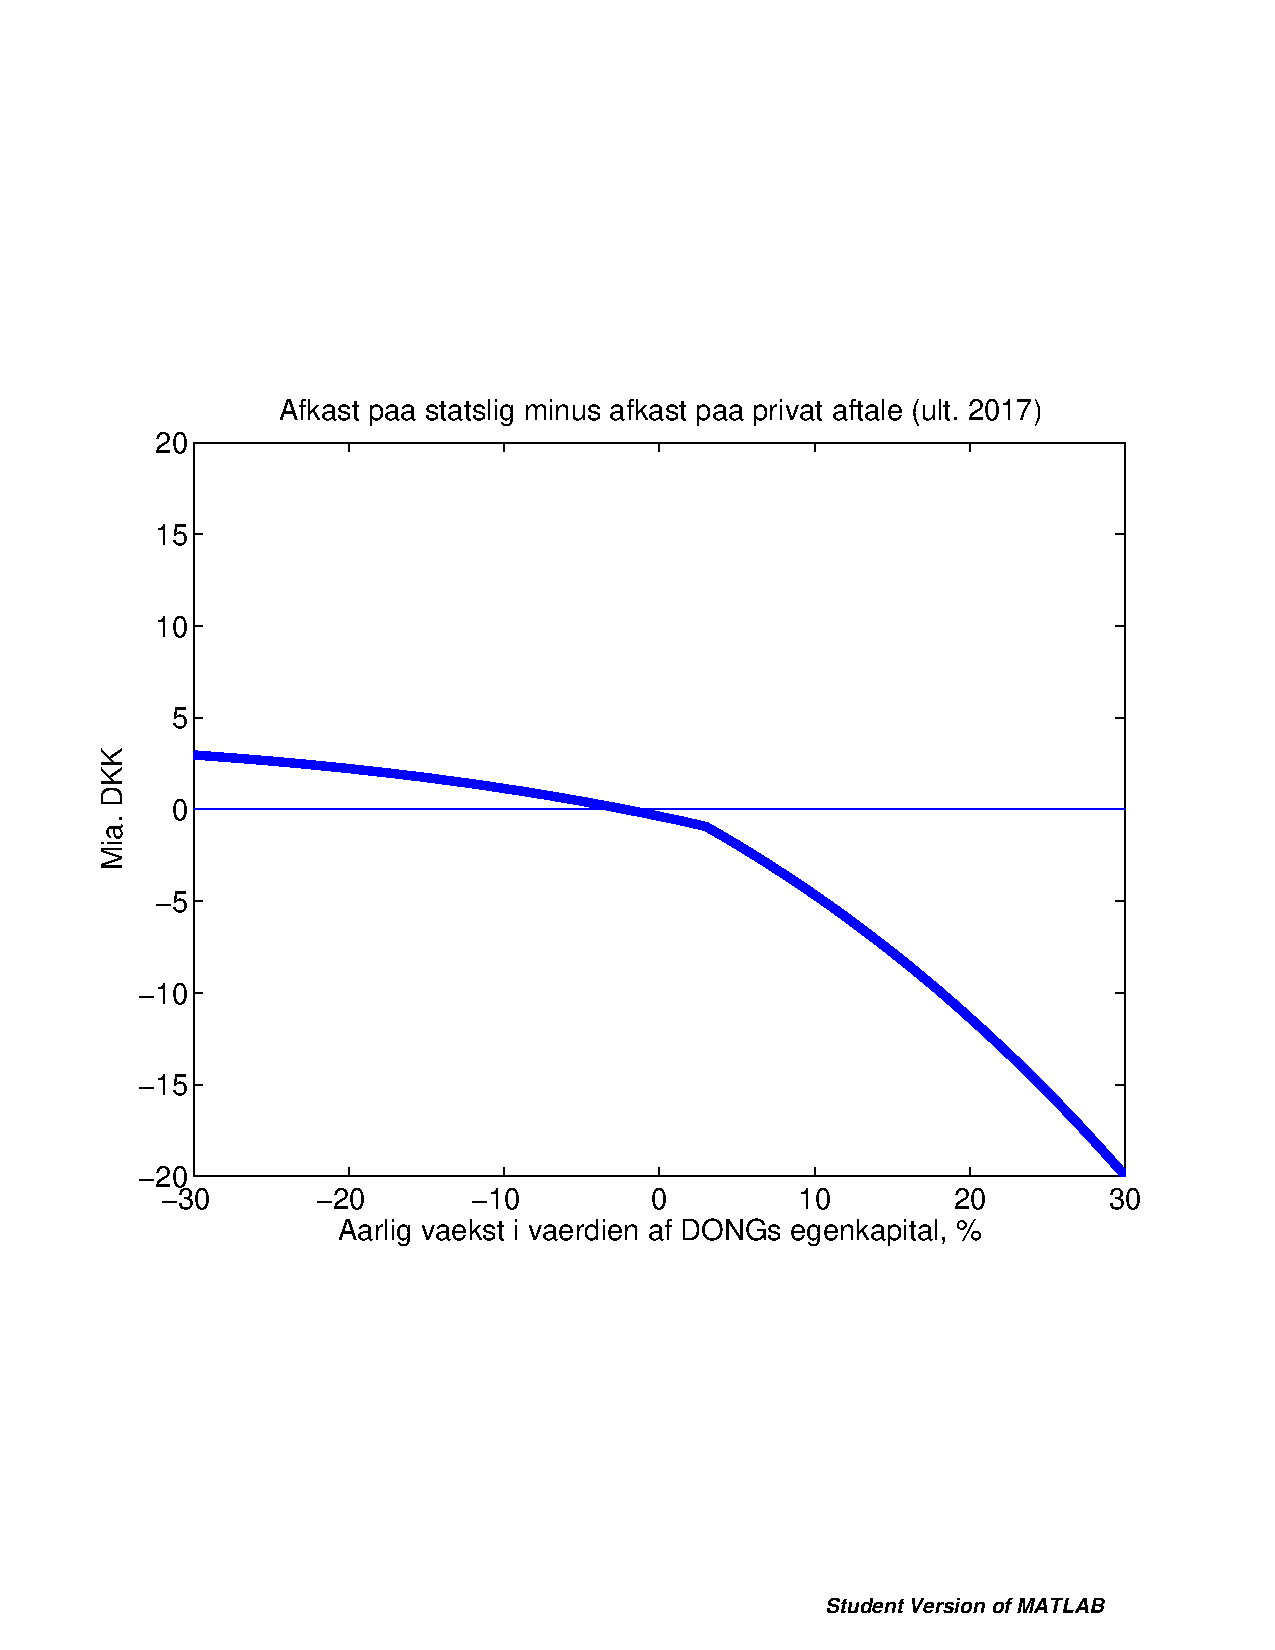
\includegraphics[scale=0.45]{../../matlab/Samfundsokonom/figs/private_less_public_deal}
%\caption{Illustration af forskellen mellem statens absolutte afkast på den indgåede private aftale og den alternative offentlig aftale som funktion af den årlige vækst i DONGs egenkapital. }
\label{fig:comp}
\end{figure}	
\end{frame}

\begin{frame}{Hvad er det forventede afkast på aftalen?}
\begin{itemize}
	\item Forventet afkast på DONG's egenkapital frem mod 2017 afgørende
	\item Kan ikke forecastes
	\item Men Monte Carlo simulation
	\item Antag DONG blev handlet til markedsprise -> daglig prisudvikling er random walk.
	\item Hvilken fordeling?
	\begin{enumerate}
		\item \textbf{13 børsnoterede europæiske electricitetsselskaber}
		\item 8 europæiske olie- og gasselskaber. 
		\item Frem til primo 2014
	\end{enumerate}
\end{itemize}
\end{frame}


\begin{frame}{Europæiske energiselskaber}
	\begin{figure}
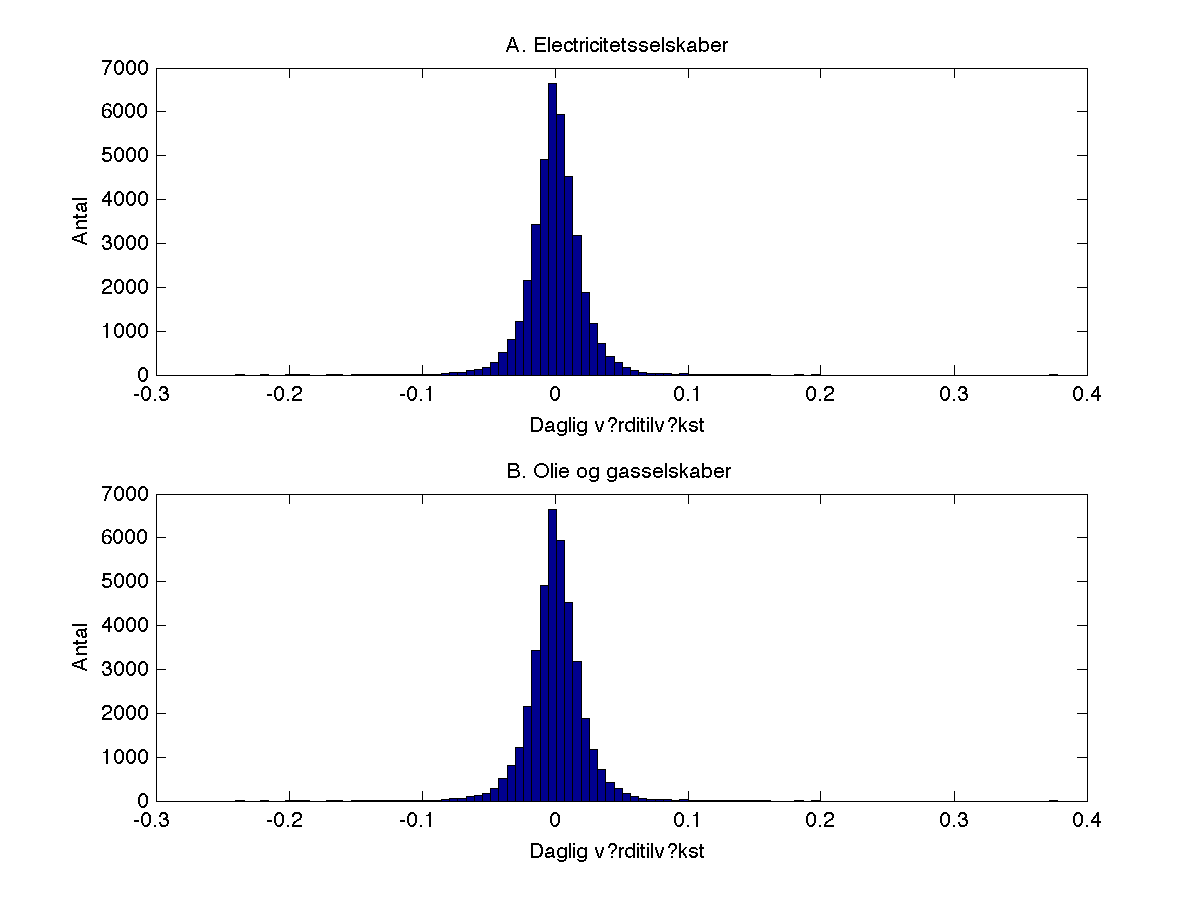
\includegraphics[scale=0.4]{../../matlab/Samfundsokonom/figs/data_hist}
%\caption{Fordeling af daglige vækstrater i Europæiske energiselskaber}
\label{fig:data_hist}
\end{figure}
\end{frame}

\begin{frame}{Fordeling af gevinst på privat aftale}
\begin{figure}
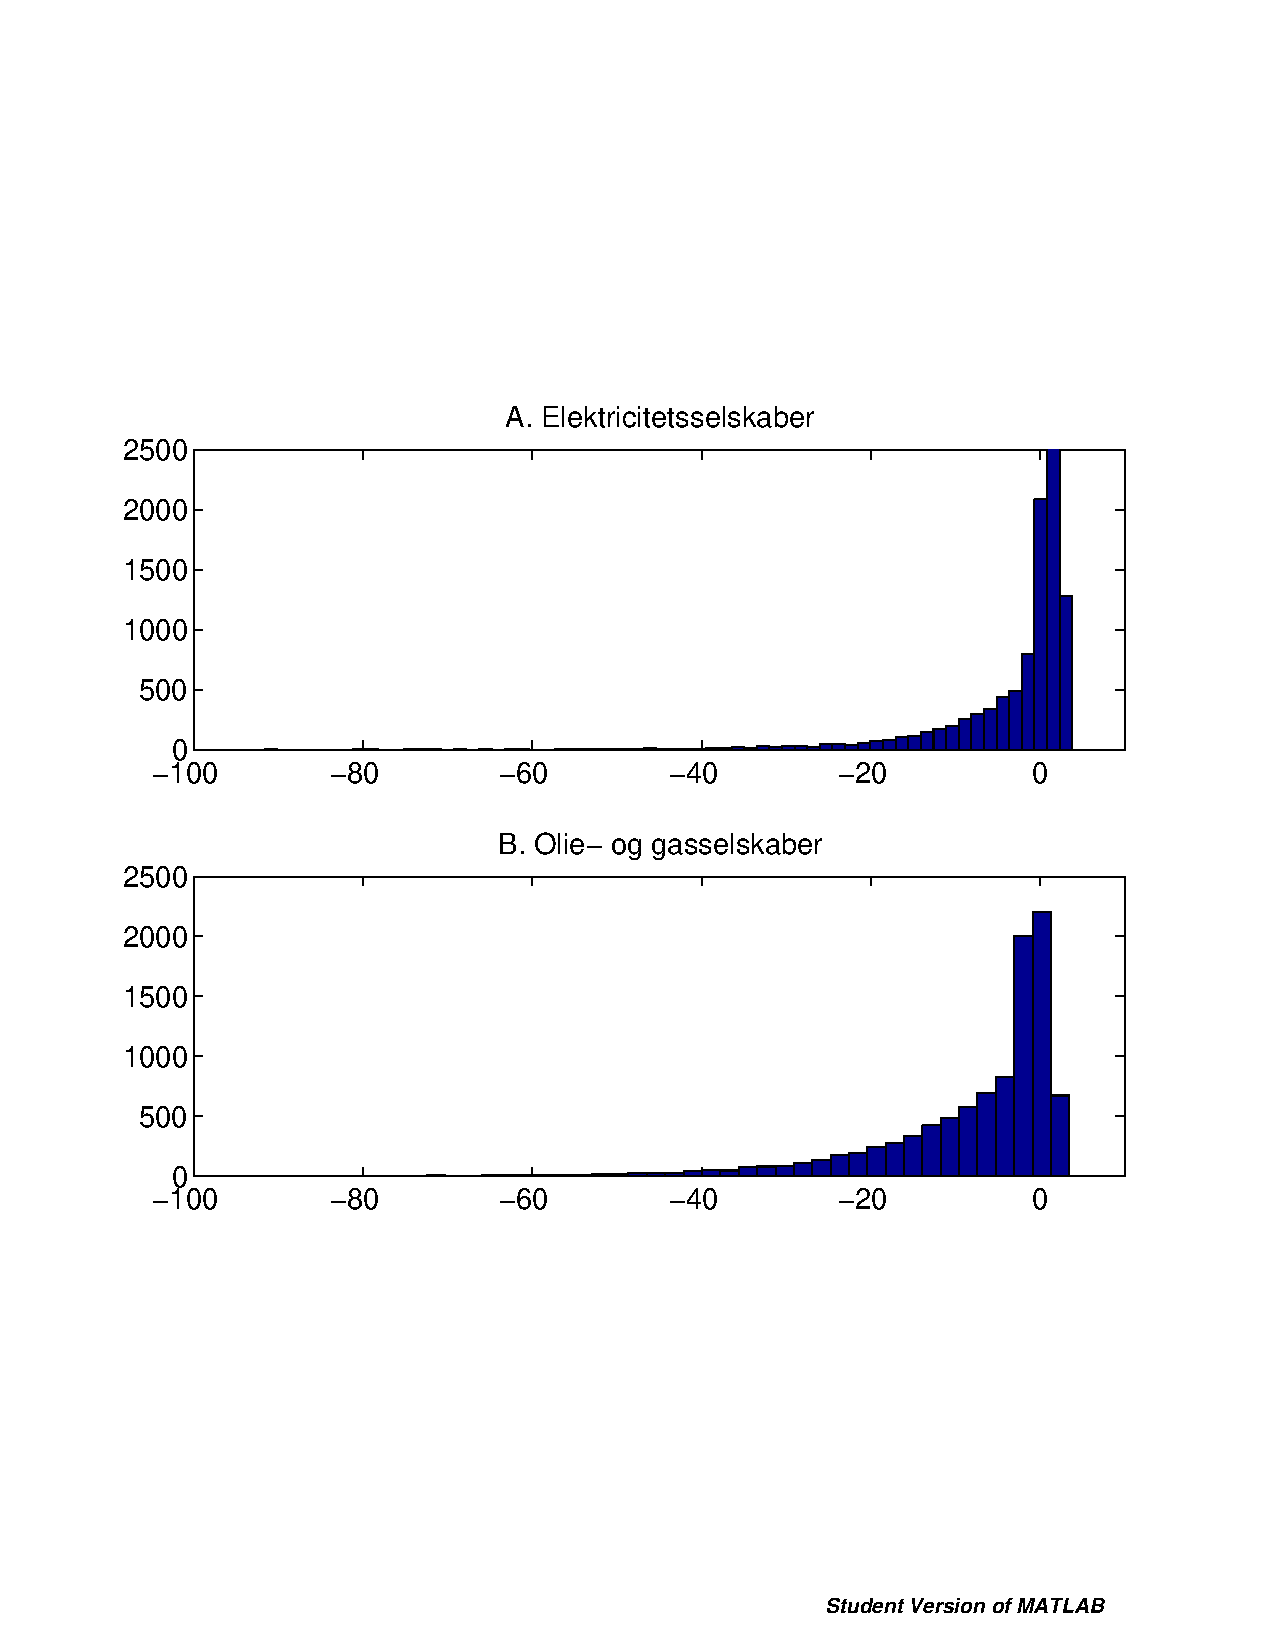
\includegraphics[scale=0.45]{../../matlab/Samfundsokonom/figs/sim_return}
\caption{Fordeling af gevinst på privat aftale ift. offentlig aftale. 10 000 simulationer. TBD }
\label{fig:sim}
\end{figure}
\end{frame}

\begin{frame}{Fordeling af gevinst på privat aftale}
\Fontvi
	\begin{table}[h]
	\caption{Fordeling af absolut gevinst på privat aftale og offentlig aftale. 10 000 simulationer. TBD}
	\label{tab:abs_fordeling}
	\begin{tabularx}{\linewidth}{cXcccccr}
	\toprule[1pt] 
	Fordeling && Gennemsnit, mia. & \multicolumn{3}{c}{Standard afvigelse, mia.}  & Sandsynlighed for gevinst\\
	& & &Total & >0 & <0 \\
	\hline 
	\emph{Offentlig aftale} \\
	%\midrule
		Europæiske elektricitetsselskaber && -0.5  & 9.1  &7.2  & 3.2  & 33.5  \% \\
	Europæiske gas og olie selskaber && 5.6  & 13.8  & 12.7  & 2.5  &58.8  \% \\
	\emph{Privat aftale} \\
		Europæiske elektricitetsselskaber && -2.4  & 2.1 &0.0 &2.1 & 0.0  \% \\
	Europæiske gas og olie selskaber && -1.2  & 1.7 & 0.0 & 1.7 &0.0 \% \\
		\bottomrule[1pt]
	\end{tabularx}
	\begin{minipage}{\linewidth}
		%\footnotesize{Noter: }
	\end{minipage}
\end{table}
\end{frame}

\begin{frame}{Fordeling af gevinst på privat aftale}
\Fontvi

\begin{table}[h]
	\caption{Fordeling af gevinst på privat aftale ift. offentlig aftale. 10 000 simulationer. TBD}
	\label{tab:rel_fordeling}
	\begin{tabularx}{\linewidth}{cXcccccr}
	\toprule[1pt]
	Fordeling && Gennemsnitsgevinst & Standard afvigelse & Sandsynlighed for gevinst\\
	\hline 
	\emph{Ekslusiv 2014 data} \\
	%\midrule
		Europæiske elektricitetsselskaber && -2.1 mia. & 8.15 mia & 58.6  \% \\
	Europæiske gas og olie selskaber && -7.0 mia. & 12.8 mia & 33.0  \% \\
	\emph{Inklusiv 2014 data} \\
		Europæiske elektricitetsselskaber && -2.1 mia. & 7.7 mia & 57.6  \% \\
	Europæiske gas og olie selskaber && -5.8 mia. & 11.2 mia & 36.4 \% \\
		\bottomrule[1pt]
	\end{tabularx}
	\begin{minipage}{\linewidth}
		%\footnotesize{Noter: }
	\end{minipage}
\end{table}
\end{frame}

\section{Robusthed}
\subsection{}


\begin{frame}{Robusthed}

\begin{itemize}
	\item \textbf{DONGs handlet over markedsprisen ?}
	\item Usikkerhed om udnyttelse af salgsret
	\item Afkastsfordeling
	\item Risiko neutralitet
\end{itemize}

	
\end{frame}

\begin{frame}{Robusthed: Initiale pris}
\Fontvi
	\begin{table}[h]
	\caption{Fordeling af gevinst på privat aftale ift. offentlig aftale. 10 000 simulationer. TBD}
	\label{tab:rel_fordeling}
	\begin{tabularx}{\linewidth}{cXcccccr}
	\toprule[1pt]
	Fordeling && Gennemsnitsgevinst & Standard afvigelse & Sandsynlighed for gevinst\\
	\hline 
	\emph{Initial markedsværdi = 24} \\
	%\midrule
		Europæiske elektricitetsselskaber && -0.6 mia. & 6.2 mia & 70.0  \% \\
	Europæiske gas og olie selskaber && -4.5 mia. & 10.2 mia & 44.0  \% \\
		\emph{Initial markedsværdi = 26} \\
	%\midrule
		Europæiske elektricitetsselskaber && -0.9 mia. & 6.5 mia & 67.1  \% \\
	Europæiske gas og olie selskaber && -5.0 mia. & 10.8 mia & 42.0  \% \\
			\emph{Initial markedsværdi = 28} \\
	%\midrule
		Europæiske elektricitetsselskaber && -1.3 mia. & 6.9 mia & 64.5  \% \\
	Europæiske gas og olie selskaber && -5.5 mia. & 11.2 mia & 39.3  \% \\
			\emph{Initial markedsværdi = 30} \\
	%\midrule
		Europæiske elektricitetsselskaber && -1.6 mia. & 7.1 mia & 62.7  \% \\
	Europæiske gas og olie selskaber && -6.3 mia. & 11.8 mia & 35.5  \% \\
				\emph{Initial markedsværdi = 31.5} \\
	%\midrule
		Europæiske elektricitetsselskaber && -1.8 mia. & 7.2 mia & 60.3  \% \\
	Europæiske gas og olie selskaber && -7.1 mia. & 12.9 mia & 33.7  \% \\

		\bottomrule[1pt]
	\end{tabularx}
	\begin{minipage}{\linewidth}
		\footnotesize{Noter: Fordeling af afkast er eksklusiv 2014 data.}
	\end{minipage}
\end{table}
\end{frame}

\begin{frame}{Robusthed}

\begin{itemize}
	\item DONGs initiale pris
	\item \textbf{Usikkerhed om udnyttelse af salgsret}
	\item Afkastsfordeling
	\item Risiko neutralitet
\end{itemize}

\end{frame}

\begin{frame}{ Usikkerhed om pris i 2017}

\begin{figure}
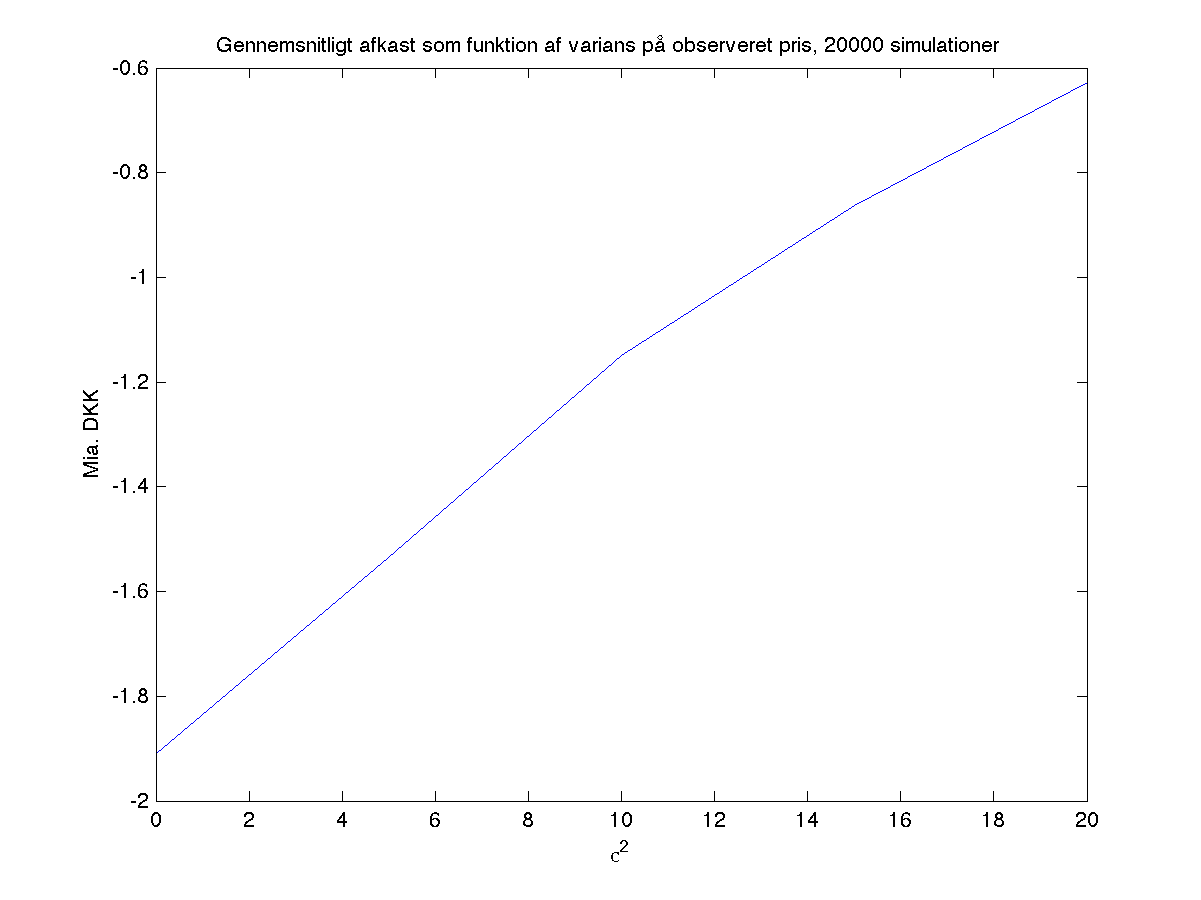
\includegraphics[scale=0.4]{../../matlab/Samfundsokonom/figs/return_variance}
%\caption{Fordeling af gevinst på privat aftale ift. offentlig aftale som funktion af $\sigma^2$. 1000 simulationer per $\sigma^2$. }
\label{fig:usikkerhed}
\end{figure}
	
\end{frame}

\begin{frame}{Robusthed}

\begin{itemize}
	\item DONGs initiale pris
	\item Usikkerhed om udnyttelse af salgsret
	\item Afkastsfordeling
	\item Risiko neutralitet
\end{itemize}

\end{frame}

\section{Konklusion}
\subsection{}

\begin{frame}{Konklusion}
\begin{itemize}
	\item Et offentligt alternativ dominerer den private aftale i forventet afkast
	\pause
	\begin{itemize}
	\item 2 mia. i benchmark simulering
	\pause 
	\item sandsynlighed for at vinde på aftale er 60 \%
	\pause 
	\item men afkaststruktur assymmetrisk
	\end{itemize}
	\pause
	\item DONG blev handlet for 88 kroner per aktie. Ikke 107 som oplyst af Finansministeriet.
	\pause 
	\item Andre argumenter for aftalen?
	\begin{itemize}
	\item Bestyrelses kompetence?
	\end{itemize}
	\pause
	\item Var aftalen virkelig \enquote{den bedst mulige} ?
	\begin{itemize}
	\item Sammenlignede FM aftalen med et offentligt alternativ?
	\item Så FT sådanne beregninger?
	\end{itemize}
\end{itemize}

\end{frame}








\section{Ekstra slides}
\subsection{}

\begin{frame}{Robbusthed: Pris}

\begin{itemize}
	\item Afkast på privat aftale
\small
\begin{align}
&P= 
\begin{dcases} 
-0.6K \prod_{i=2014}^{2017} (1+g_i)+0.6\frac{K}{V_H+K}(V_0+K)(1+r)^n +\Omega \\ 
\text{     hvis    } K\prod_{i=2014}^{2017}(1+g_k)>(V_0+K)\frac{K}{V_H+K}(1+r)^n \nonumber \\
\text{ $\Omega$} &\text{  ellers } \nonumber
\end {dcases} \\
\end{align}
\item Where 

\begin{align}
	\Omega=\left(\frac{s_0 V_H}{V_H+K}(V_0+K)-s_0V_0 \right) (1+r)^n \nonumber
\end{align}

\end{itemize}

\end{frame}

\end{document}